\chapter{Algoritmi}
\label{Geom_Algos}
%
\section{Parsificazione}
%
\subsection{Introduzione}
La parsificazione o analisi sintattica è un processo che analizza un flusso continuo di dati in ingresso (letti per esempio da un file o una tastiera) in modo da determinare la correttezza della sua struttura grazie ad una data grammatica formale. Un \textit{parser} è un programma che esegue questo compito. Nella maggior parte dei casi, l'analisi sintattica opera su una sequenza di \textit{token} in cui l'analizzatore lessicale spezzetta l'input.
%
\subsection{Parsificazione del formato RDF}
Nel lavoro svolto è stato creato un algoritmo per pardificare i file di tipo \ac{RDF} che descrivono superfici complesse. Purtroppo, come precedentemente detto, non esiste uno standard universalmente riconosciuto per questo formato. Creare dunque un \textit{parser} o definire un generatore di parser è arduo. Si è quindi optato per la creazione di un \textit{parser} che rilevi solo i nodi (\texttt{[NODES]}), li salvi temporaneamente e, dopo aver immagazzinato anche i dati relativi agli elementi (\texttt{[ELEMENTS]}), instanzi un oggetto \textit{mesh}, composto dai nodi dichiarati nella sezione elementi. Gli altri parametri non sono stati considerati.\\

Come verrà richiamato nelle conclusioni, l'importanza di definire uno standard per il formato \ac{RDF} è di cruciale importanza. In questo modo si potrà creare un generatore di parser con una grammatica e un lessico ben definiti, nonché aumentarne l'efficienza e la stabilità.
%
%
\section{\textit{Bounding Volume Hierarchy}}
%
\subsection{Introduzione}
Una \ac{BVH} è una struttura ad albero su un insieme di oggetti geometrici. Tutti gli oggetti geometrici sono raccolti in volumi limite che formano i nodi fogliari dell'albero. Questi nodi vengono quindi raggruppati come piccoli insiemi e racchiusi in volumi di delimitazione più grandi. Questi, a loro volta, sono ancora raggruppati e racchiusi in altri volumi di delimitazione più grandi in modo ricorsivo, risultando infine in una struttura ad albero con un singolo volume di delimitazione nella parte superiore dell'albero. Le gerarchie di volumi limitanti vengono utilizzate per supportare in modo efficiente diverse operazioni su insiemi di oggetti geometrici, come ad esempio il rilevamento delle collisioni.

Sebbene il \textit{wrapping} degli oggetti nei volumi di delimitazione e l'esecuzione di test di collisione su di essi prima del test della geometria dell'oggetto stesso semplifichino i test e possano comportare miglioramenti significativi delle prestazioni, è ancora in corso lo stesso numero di test a coppie tra volumi di delimitazione. Organizzando i volumi di delimitazione in una gerarchia di volumi di delimitazione, la complessità temporale (il numero di test eseguiti) può essere ridotta logaritmicamente nel numero di oggetti. Con una tale gerarchia in atto, durante i test di collisione, i volumi secondari non devono essere esaminati se i loro volumi principali non sono intersecati.
%
\subsection{\textit{Minimum Bounding Box}}
In geometria, il rettangolo minimo o più piccolo (o \ac{MBB}) per racchiudere un insieme di punti $S$ in $N$ dimensioni è l'rettangolo con la misura più piccola (area, volume o ipervolume in dimensioni superiori) all'interno del quale si trovano tutti i punti.  Il termine "iper-rettangolo (o più semplicemente \textit{box}) deriva dal suo utilizzo nel sistema di coordinate cartesiane, dove viene effettivamente visualizzato come un rettangolo (caso bidimensionale), parallelepipedo rettangolare (caso tridimensionale), ecc. Nel caso bidimensionale viene chiamato rettangolo di delimitazione minimo.
%
\subsubsection{\textit{Axis Aligned Bounding Box}}
Il \ac{MBB} allineato agli'assi (\ac{AABB}) per un determinato set di punti è il rettangolo di delimitazione minimo soggetto al vincolo che i bordi del rettangolo sono paralleli agli assi cartesiani. È il prodotto cartesiano di $N$ intervalli ciascuno dei quali è definito da un valore minimo e un valore massimo della coordinata corrispondente per i punti in $S$.

I rettangoli di delimitazione minimi allineati all'asse vengono utilizzati per determinare la posizione approssimativa di un oggetto e come descrittore molto semplice della sua forma. Ad esempio, nella geometria computazionale e nelle sue applicazioni quando è necessario trovare intersezioni nel set di oggetti, il controllo iniziale sono le intersezioni tra i loro \ac{MBB}. Dato che di solito è un'operazione molto meno costosa del controllo dell'intersezione effettiva (perché richiede solo confronti di coordinate), consente di escludere rapidamente i controlli delle coppie che sono molto distanti.

\begin{figure}[h]
	\centering
	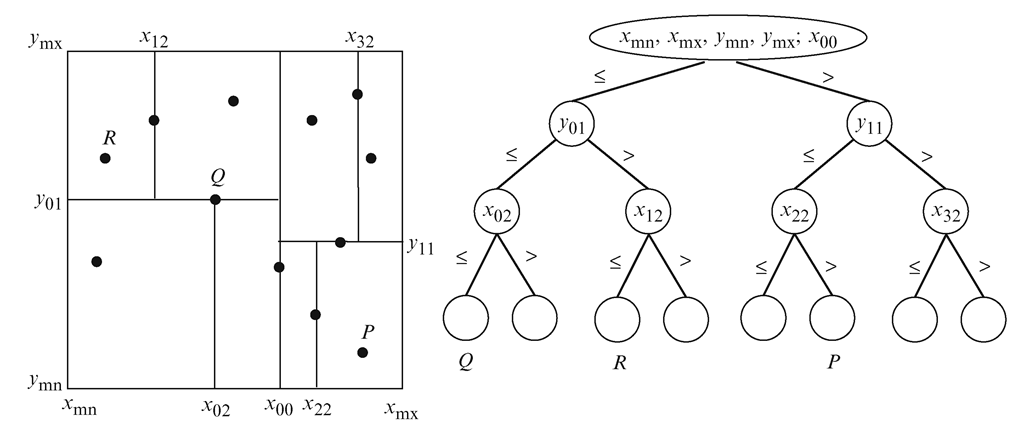
\includegraphics[width=\linewidth]{Figures/AABB}
	\caption{Esempio di albero di tipo \ac{AABB}.}
	\label{AABB}
\end{figure}
%
\subsubsection{\textit{Arbitrarily Oriented Bounding Box}}
Il \ac{MBB} orientato arbitrariamente (\ac{AOBB}) è il rettangolo di delimitazione minimo, calcolato senza vincoli per quanto riguarda l'orientamento del risultato. Gli algoritmi del rettangolo di delimitazione minimo basati sul metodo dei calibri rotanti possono essere utilizzati per trovare l'area di delimitazione dell'area minima o del perimetro minimo di un poligono convesso bidimensionale in tempo lineare e di un punto bidimensionale impostato nel tempo impiegato costruire il suo scafo convesso seguito da un calcolo del tempo lineare. Un algoritmo di pinze rotanti tridimensionali può trovare il rettangolo di delimitazione orientato arbitrariamente sul volume minimo di un punto tridimensionale impostato in tempo cubo.
%
\subsubsection{\textit{Object Oriented Bounding Box}}
Nel caso in cui un oggetto abbia un proprio sistema di coordinate locale, può essere utile memorizzare un rettangolo di selezione relativo a questi assi, che non richiede alcuna trasformazione quando cambia l'orientazione dell'oggetto stesso.

%\begin{figure}[h]
%	\centering
%	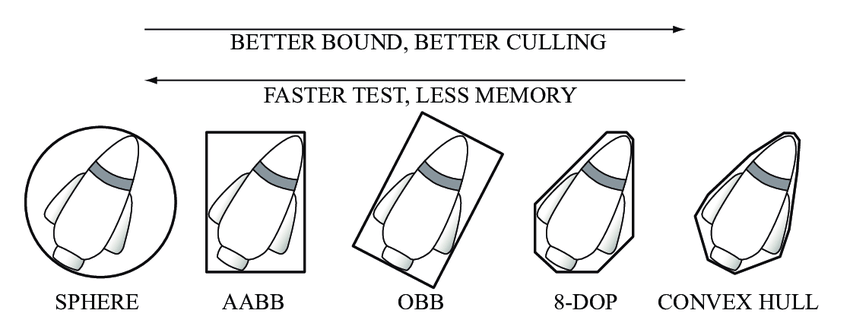
\includegraphics[width=0.9\linewidth]{Figures/BB}
%	\caption{Tipi di \ac{BVH}.}
%	\label{BB}
%\end{figure}
%
\subsection{Intersezione tra Alberi AABB}

Per il rilevamento delle collisioni tra oggetti in due dimensioni, l'intersezione tra alberi di tipo \ac{AABB}, è l'algoritmo più veloce per determinare se le due entità di gioco si sovrappongono o meno, e in che parti. Nello specifico, ciò consiste nel controllare le posizioni delle \textit{i}-esime \ac{BB} nello spazio delle coordinate bidimensionali per vedere se si sovrappongono.

Il vincolo di allineamento dei rettangoli agli assi è presente per motivi di prestazioni, infatti, l'area di sovrapposizione tra due riquadri non ruotati può essere controllata solo con confronti logici. Mentre i riquadri ruotati richiedono ulteriori operazioni trigonometriche, che sono più lente da calcolare. Inoltre, se si hanno entità che possono ruotare, le dimensioni dei rettangoli e/o sotto-rettangoli dovranno modificarsi in modo da avvolgere ancora l'oggetto o si dovrà optare per un altro tipo di geometria di delimitazione, come le sfere (che sono invarianti alla rotazione).

Nel caso specifico, l'ombra dello pneumatico sarà rappresentata da un albero di tipo \ac{AABB} con una sola foglia. Ovvero si andrà a rappresentare lo pneumatico con una \ac{BB} avente lati uguali e rappresentanti il massimo ingombro che può avere nello spazio. Si andrà inoltre ad incrementare del 10\% ognuno di questi lati in modo da tenere conto dell'angolo di camber, che portrebbe portare i punti di campionamento del terreno fuori dall'ombra. La strada, contrariamente al pneumatico, verrà tenuta come riferimento assoluto. In altre parole, una volta effettuato la parsificazione del file \ac{RDF}, verrà calcolato l'albero di tipo \ac{AABB}. Lo pneumatico si muoverà all'interno della \textit{mesh} e la sua ombra verrà ricalcolata e intersecata con l'albero \ac{AABB} per ottenere tutti i triangoli in corrispondenza della stessa.

Volendo intersecare due semplici \ac{BB}, quali $A = \left[ \texttt{A.minX}, \texttt{A.maxX} ;  \texttt{A.minY}, \texttt{A.maxY} \right]$ e $B = \left[ \texttt{B.minX}, \texttt{B.maxX} ;  \texttt{B.minY}, \texttt{B.maxY} \right]$, verrà usata la seguente funzione.
\begin{pseudoc}
	function intersect(A, B) {
		return (A.minX <= B.maxX && A.maxX >= B.minX) &&
					 (A.minY <= B.maxY && A.maxY >= B.minY);
	}
\end{pseudoc}
\noindent
Volendo intersecare un albero di tipo \ac{AABB} e una semplice \ac{BB}, basterà ripetere a più step la funzione precedente lungo i rami dell'albero. Una volta arrivati a una o più foglia avremo tutti gli oggetti (o triangoli nel caso specifico) che sono posti in corrispondenza della \ac{BB} (od ombra dello pneumatico nel caso specifico). Questi triangoli verranno poi usati per determinare il piano strada locale e il punto di contatto virtuale dello pneumatico.

È imporatante notare che il metodo appena visto, presenta numerosi vantaggi.
\begin{itemize}
	\item Riduzione del numero di comparazioni da effettuare per ottenere l'intersezione \ac{BB}-albero \ac{AABB}. Infatti, la \textit{mesh} può contenere decine di migliaia di trangoli, il metodo presentato consente di ridurre logarirmicamente il numero di comparazioni necessarie per ottenere il risultato.
	\item Riduzione del numero di trangoli da processare per ottenere il piano strada locale e il punto di contatto virtuale dello pneumatico. Infatti, vengono solamente processati quelli posti in corrispondenza del'ombra dello pneumatico.
\end{itemize}
%
\section{Algoritmi Geometrici}
%
\subsection{Introduzione}
La geometria computazionale è la branca dell'informatica che studia le strutture dati e gli algoritmi efficienti per la soluzione di problemi di natura geometrica e la loro implementazione al calcolatore. Storicamente, è considerato uno dei campi più antichi del calcolo, anche se la geometria computazionale moderna è uno sviluppo recente. La ragione principale per lo sviluppo della geometria computazionale è stata dovuta ai progressi compiuti nella computer grafica, \ac{CAD}, \ac{CAM} e nella visualizzazione matematica. Ad oggi, le applicazioni della geometria computazionale si trovano nella robotica, nella progettazione di circuiti integrati, nella visione artificiale, in \ac{CAE} e nel \ac{GIS}. I rami principali della geometria computazionale sono:
\begin{itemize}
	\item \textit{Calcolo combinatorio} (o \textit{geometria algoritmica}), che si occupa di oggetti geometrici come entità discrete. Ad esempio, può essere utilizzato per determinare il poliedro o il poligono più piccolo che contiene tutti i punti forniti, o più formalmente, dato un insieme di punti, si deve determinare il più piccolo insieme convesso che li contenga tutti (problema dell'inviluppo convesso).
	\item \textit{Geometria di calcolo} numerica (o \ac{CAGD}), che si occupa principalmente di rappresentare oggetti del mondo reale in forme adatte per i calcoli informatici nei sistemi \ac{CAD} e \ac{CAM}. Questo ramo può essere visto come uno sviluppo della geometria descrittiva ed è spesso considerato un ramo della computer grafica o del \ac{CAD}. Entità importanti di questo ramo sono superfici e curve parametriche, come ad esempio le \textit{spline} e \textit{curve di Bézier}.
\end{itemize}

In questo capitolo tutti gli algoritmi che verranno utilizzati in seguito durante l'analisi geometrica dell'intersezione tra pneumatico e superficie stradale saranno trattati. Questi algoritmi sono la soluzione di alcuni semplici ma molto importanti problemi, che devono essere risolti in modo efficiente. In particolare le intersezioni tra:
\begin{itemize}
	\item punto e segmento (sul piano);
	\item punto e circonferenza (sul piano);
	\item raggio e circonferenza (sul piano);
	\item raggio e triangolo (sullo spazio);
\end{itemize}
saranno esaminati al fine di trovare la massima prestazione in termini di efficienza computazionale.
%
\subsection{Intersezione tra Entità Geometriche}
%
\subsubsection{Punto-Segmento}
Dato un punto $P = (x_p, y_p)$ e un segmento definito da due punti $A = (x_A, y_B)$ e $B = (x_B, y_B)$.

\begin{figure}[h!]
	\centering
	\begin{tikzpicture}
	\def\r{2};
	\coordinate (P) at (0.3,0.7);
	\coordinate (A) at (-2.0,0.0);
	\coordinate (B) at (+2.0,0.0);
	\draw[fill] (A) circle [radius=1pt] node[above] {$A$};
	\draw[fill] (B) circle [radius=1pt] node[above] {$B$};
	\draw[fill] (P) circle [radius=1pt] node[above] {$P$};
	\draw[thick](A) -- (B);
	\end{tikzpicture}
	\caption{Schema grafico per l'intersezione punto-segmento}
\end{figure}
\noindent
Per determinare se il punto $P$ è intermo al segmento si eseguiranno i seguenti step.
\begin{enumerate}
	\item Creazione di un vettore $\vv{AB}$ e di un vettore $\vv{AP}$.
	\item Calcolo il prodotto vettoriale  $\vv{P_1P_2} \times  \vv{PP_1}$, se il modulo del vettore risultante è nullo allora il punto $P$ appartiene al segmento considerato.
	\item Calcolo il prodotto scalare tra $\vv{AB}$ e $\vv{AP}$. Se è nullo allora il punto $P$ è coincidente a $A$, se è pari al modulo di $\vv{AB}$ allora il punto $P$ è coincidente a $B$, se è compreso tra 0 il modulo di $\vv{AB}$, allora il punto $P$ giace all'interno del segmento considerato.
\end{enumerate}
Il codice che esegue questo tipo di test è riportato in \figurename{ \ref{pointsegment}}

\begin{figure}[h!]
	\hfill
	\begin{subfigure}{.45\textwidth}
		\centering
		\begin{tikzpicture}
		\coordinate (P0) at (0.3,0.7);
		\coordinate (P3) at (-0.7,0);
		\coordinate (A) at (-2.0,0.0);
		\coordinate (B) at (+2.0,0.0);
		\draw[fill] (P0) circle [radius=1pt] node[above] {\texttt{0}};
		\draw[fill] (A) circle [radius=1pt] node[above] {\texttt{1}};
		\draw[fill] (B) circle [radius=1pt] node[above] {\texttt{2}};
		\draw[fill] (P3) circle [radius=1pt] node[above] {\texttt{3}};
		\draw[thick](A) -- (B);
		\end{tikzpicture}
		\caption{Output tipo \texttt{integer}}
	\end{subfigure}
	\hfill
	\begin{subfigure}{.45\textwidth}
		\centering
		\begin{tikzpicture}
		\coordinate (P0) at (0.3,0.7);
		\coordinate (P3) at (-0.7,0);
		\coordinate (A) at (-2.0,0.0);
		\coordinate (B) at (+2.0,0.0);
		\draw[fill] (P0) circle [radius=1pt] node[above] {\texttt{false}};
		\draw[fill] (A) circle [radius=1pt] node[above] {\texttt{true}};
		\draw[fill] (B) circle [radius=1pt] node[above] {\texttt{true}};
		\draw[fill] (P3) circle [radius=1pt] node[above] {\texttt{true}};
		\draw[thick](A) -- (B);
		\end{tikzpicture}
		\caption{Output tipo \texttt{bool}}
	\end{subfigure}
	\hfill
	\caption{Schemi per l'output dell'intersezione punto-segmento.}
\end{figure}

\begin{figure}[h!]
	\hfill
	\begin{subfigure}[t]{.45\linewidth}
	\raggedright
	Output tipo \texttt{integer}\\
	\vspace{.5em}
	\begin{pseudoc}
	if (AB.cross(AP) > epsilon) { return 0 }
	KAP = AB.dot(AP)
	if ( KAP      < -epsilon ) { return 0 }
	if ( abs(KAP) < epsilon  ) { return 1 }
	KAB = AB.dot(AB)
	if ( KAP > KAB )  { return 0 }
	if ( abs(KAP - KAB) < epsilon ) { return 2 }
	return 3 // The point is on the segment
	\end{pseudoc}
	\end{subfigure}
	\hfill
	\begin{subfigure}[t]{.45\textwidth}
	\raggedright
	Output tipo \texttt{bool}\\
	\begin{pseudoc}
	if (AB.cross(AP) > epsilon) { return false }
	KAP = AB.dot(AP)
	if ( KAP      < -epsilon ) { return false }
	if ( abs(KAP) < epsilon  ) { return true }
	KAB = AB.dot(AB)
	if ( KAP > KAB )  { return false }
	if ( abs(KAP - KAB) < epsilon ) { return true }
	return true // The point is on the segment
	\end{pseudoc}
	\end{subfigure}
	\hfill
	\caption{Schema del codice per l'intersezione punto-segmento.}
	\label{pointsegment}
\end{figure}
%
\subsubsection{Punto-Cerchio}
Having a circle with center $C = (x_c, y_c)$ and radius $r$, the problem consists in finding out whether a query point $P = (x_p, y_p)$ is inside, outside or on the circle.
%
\begin{figure}
	\centering
	\begin{tikzpicture}
	\def\r{2};
	\coordinate (C) at (0,0) node[above left] {$C$};
	\draw[thick, fill=gray!10](C) circle (\r);
	\coordinate (P) at (-0.5,-1.5);
	\draw[fill] (C) circle [radius=1pt];
	\draw[fill] (P) circle [radius=1pt];
	\draw(C) -- (P)  node[above left] {$P$} node[pos=0.5, right] {$d$};
	\draw(C) -- ({sqrt(\r)},{sqrt(\r)}) node[pos=0.4, above] {$r$};
	\end{tikzpicture}
	\caption{Point-circle intersection problem scheme.}
\end{figure}
%
The solution to the problem is simple: the distance between the circle center $C$ and the query point $P$ is given by the \textit{Pythagorean theorem} as
\begin{equation}
	d=\sqrt{(x_p-x_c)^2 + (y_p-y_c)^2}
\end{equation}
The query point $P$ is \textit{inside} the circle if $d<r$, on the circle if $d = r$, and \textit{outside} the circle if $d > r$. Little work can be saved by comparing $d^2$ with $r^2$ instead: the point $P$ is \textit{inside} the circle if $d^2<r^2$, on the circle if $d^2 = r^2$, and \textit{outside} the circle if $d^2 > r^2$. Thus, the final comparison will be between the number $(x_p-x_c)^2 + (y_p-y_c)^2$ and $r^2$.\\
The \textit{inputs} of the point-circle intersection algorithm are:
\begin{itemize}
	\item the circle center $C = (x_c, y_c)$;
	\item the circle radius $r$;
	\item a query point $P=(x_p, y_p)$.
\end{itemize}
The \textit{output} could be an integer which value is:
\begin{itemize}
	\item 0 if the point is outside;
	\item 1 if the point is inside;
	\item 2 if the point is on the circle.
\end{itemize}
Another option could be a boolean which value is:
\begin{itemize}
	\item false if the point is outside;
	\item true if the point is inside or on the circle.
\end{itemize}
%
\begin{figure}
\hfill
	\begin{subfigure}{.45\textwidth}
	\centering
	\begin{tikzpicture}
	\def\r{2};
	\coordinate (C) at (0,0);
	\draw[thick, fill=gray!10](C) circle (\r);
	\draw[fill] (0,-0.5) circle [radius=1pt] node[above left] {\texttt{1}};
	\draw[fill] (-\r,0) circle [radius=1pt] node[above left] {\texttt{2}};
	\draw[fill] (3,0) circle [radius=1pt] node[above left] {\texttt{0}};
	\end{tikzpicture}
	\caption{Output tipo \texttt{integer}}
	\end{subfigure}
\hfill
\begin{subfigure}{.45\textwidth}
	\centering
	\begin{tikzpicture}
	\def\r{2};
	\coordinate (C) at (0,0);
	\draw[thick, fill=gray!10](C) circle (\r);
	\draw[fill] (0,-0.5) circle [radius=1pt] node[above left] {\texttt{true}};
	\draw[fill] (-\r,0) circle [radius=1pt] node[above left] {\texttt{true}};
	\draw[fill] (3,0) circle [radius=1pt] node[above] {\texttt{false}};
	\end{tikzpicture}
	\caption{Output tipo \texttt{bool}}
\end{subfigure}
\hfill
\caption{Schemi per l'output dell'intersezione punto-cerchio.}
\end{figure}
On \figurename{ \ref{Pointcircle}} the schemes for the point-circle intersection algorithm with integer and boolean outputs are reported.\\
%
\begin{figure}[htbp]
\hfill
	\begin{subfigure}[t]{.45\linewidth}
	\raggedright
	Output tipo \texttt{integer}\\
	\vspace{.5em}
	\begin{pseudoc}
	d = (x_p-x_c)^2 + (y_p-y_c)^2
	if (d > r^2) { return  0}
	else if (d < r^2) { return 1 }
	else { return 2} // d = r^2
	\end{pseudoc}
	\end{subfigure}
\hfill
	\begin{subfigure}[t]{.45\textwidth}
	\raggedright
	Output tipo \texttt{bool}\\
	\vspace{.5em}
	\begin{pseudoc}
	d = (x_p-x_c)^2 + (y_p-y_c)^2
	if (d > r^2) { return  true}
	else { return false} // d <= r^2
	\end{pseudoc}	
	\end{subfigure}
\hfill
\caption{Schemi per l'intersezione punto-cerchio.}
\label{Pointcircle}
\end{figure}
%
\subsubsection{Piano-Cerchio}
%
\subsubsection{Piano-Triangolo}

\subsubsection{Raggio-Triangolo}
Having a triangle with vertices $(V_1,V_2,V_3)$ and a ray $R$ with origin $R_O$ and direction $R_D$, the problem consists in finding out whether the ray hits or not the triangle and if so, where is the intersection point $P$.
%
\begin{figure}[htbp]
	\centering
	\begin{tikzpicture}
	\coordinate [label=left:$V_1$] (A) at (-1,-0.5);
	\coordinate [label=above:$V_2$] (B) at (1,1);
	\coordinate [label=right:$V_3$] (C) at (2.2,-1);
	\draw[fill=gray!10] (A) -- (B) -- (C) -- (A);
	\def\xp{0.4};
	\def\yp{-0.2};
	\def\xd{-1};
	\def\yd{1};
	\def\mag{1.7};
	\coordinate [label=above right:$P$] (P) at (\xp,\yp);
	\coordinate [label={[shift={(0.1,0.1)}]$R_D$}] (RD) at (\xp+\xd,\yp+\yd);
	\coordinate [label=above:$R_O$] (RO) at (\xp+\xd*\mag,\yp+\yd*\mag);
	\draw[fill] (P) circle [radius=1pt];
	\draw[fill] (RO) circle [radius=1pt];
	\draw[-stealth] (RO) -- (RD);
	\draw[dashed] (RD) -- (P);
	\end{tikzpicture}
	\caption{Ray-triangle intersection problem scheme.}
\end{figure}
%
Over the last decades, plenty of algorithms for solving this problem had been purposed, so there are several solutions to the ray/triangle or ray-triangle intersection problem. Three of the most relevant algorithms are:
\begin{itemize}
	\item \textit{Badouel} algorithm;
	\item \textit{Segura} algorithm;
	\item \textit{M\"oller-Trumbore} algorithm.
\end{itemize}
As \citeauthor{RayTriangle} states in \cite{RayTriangle}, the M\"oller-Trumbore's is the faster algorithm when the normal and/or the projection plane have not been previously stored, as in this thesis.\\
%
\begin{figure}[htbp]
	\centering
	\hfill
	\begin{subfigure}[t]{.3\linewidth}
		\begin{tikzpicture}
			\coordinate (O) at (0,0,0);
			\def\axisl{3}
			\draw[-stealth] (O) -- (\axisl,0,0) node[below]{$x$};
			\draw[-stealth] (O) -- ({sqrt(\axisl)},{sqrt(\axisl)},0) node[above]{$y$};
			\draw[-stealth] (O) -- (0,\axisl,0) node[left]{$z$};
			
			\coordinate [label=below:$V_1$] (V1) at ({\axisl/1.5},0,0);
\coordinate [label=above:$V_2$] (V2) at ({sqrt(\axisl)/1.5},{sqrt(\axisl)/1.5},0);
\coordinate [label=above:$V_3$] (V3) at (0,0,0);
			
			\draw[fill=gray!10] (V1) -- (V2) -- (V3) -- (V1);

		\end{tikzpicture}
	\end{subfigure}
\hfill
\begin{subfigure}[t]{.3\linewidth}
	\begin{tikzpicture}
			\coordinate (O) at (0,0,0);
			\def\axisl{3}
		\draw[-stealth] (O) -- (\axisl,0,0) node[below]{$x$};
\draw[-stealth] (O) -- ({sqrt(\axisl)},{sqrt(\axisl)},0) node[above]{$z$};
\draw[-stealth] (O) -- (0,\axisl,0) node[left]{$y$};
			
			\coordinate [label=below:$V_1$] (V1) at ({\axisl/1.5},0,0);
			\coordinate [label=above:$V_2$] (V2) at ({sqrt(\axisl)/1.5},{sqrt(\axisl)/1.5},0);
			\coordinate [label=above:$V_3$] (V3) at (0,0,0);
			

			
			\draw[fill=gray!10] (V1) -- (V2) -- (V3) -- (V1);

	\end{tikzpicture}
\end{subfigure}
\hfill
\begin{subfigure}[t]{.3\linewidth}
	\begin{tikzpicture}
		\coordinate (O) at (0,0,0);
		\def\axisl{3}
		\draw[-stealth] (O) -- (\axisl,0,0) node[below]{$\alpha$};
		\draw[-stealth] (O) -- ({sqrt(\axisl)},{sqrt(\axisl)},0) node[above]{$\beta$};
		\draw[-stealth] (O) -- (0,\axisl,0) node[left]{$\gamma$};
		
		\coordinate [label={[below,font=\tiny]:$1$}] (V1) at ({\axisl/1.5},0,0);
		\coordinate [label={[shift={(-0.1,0.0)},font=\tiny]:$1$}] (V2) at ({sqrt(\axisl)/1.5},{sqrt(\axisl)/1.5},0);
		\coordinate (V3) at (0,0,0);
		
		\draw[fill=gray!10] (V1) -- (V2) -- (V3) -- (V1);
	\end{tikzpicture}
\end{subfigure}
\hfill
\caption{Transformation and base change of ray in M\"oller-Trumbore algorithm.}
\end{figure}

The inputs of the M\"oller-Trumbore algorithm are:
\begin{itemize}
	\item Triangle vertices $(V_1, V_2, V_3)$;
	\item Segment points $(Q_1, Q_2)$.
\end{itemize}
%
\begin{figure}[htbp]
\hfill
	\begin{subfigure}[t]{.4\linewidth}
		\raggedright
		\textit{With back-face culling}\\
		\vspace{.5em}
		$Q = Q_2 - Q_1$\\
		$E_1 = V_2 - V_1$\\
		$E_2 = V_3 - V_1$\\
		$A = Q \times E_2$\\
		$D = A \cdot E_1$\\
		$\mathbf{if} \, (D > \varepsilon) \{$\\
		\quad $T = Q_1 - V_1$\\
		\quad $u = A \cdot T$\\
		\quad $\mathbf{if} \, (u < 0.0 \, || \, u > D) \{$\\
		\quad \quad $\mathbf{return \, false}$\\
		\quad $\}$\\
		\quad $B = T \times E_1$\\
		\quad $v = B \cdot Q$\\
		\quad $\mathbf{if} \, (v < 0.0 \, || \, u + v > D) \{$\\
		\quad \quad $\mathbf{return \, false}$\\
		\quad $\}$\\
		$\} \, \mathbf{else \, if} \, (D < -\varepsilon) \{$\\
		\quad $T = Q_1 - V_1$\\
		\quad $u = A \cdot T$\\
		\quad $\mathbf{if} \, (u > 0.0 \, || \, u < D) \{$\\
		\quad \quad $\mathbf{return \, false}$\\
		\quad $\}$\\
		\quad $B = T \times E_1$\\
		\quad $v = B \cdot Q$\\
		\quad $\mathbf{if} \, (v > 0.0 \, || \, u + v < D) \{$\\
		\quad \quad $\mathbf{return \, false}$\\
		\quad $\}$\\
		$\} \, \mathbf{else} \, \{$\\
		\quad $\mathbf{return \, false}$\\
		$\}$\\
		$D_{inv} = 1.0 / D$\\
		$t = (B \cdot E_2) * D_{inv}$\\
		$\mathbf{if} \, (t > 0.0) \{$\\
		\quad $P = Q + D * t$\\
		\quad $\mathbf{return \, true}$\\
		$\} \, \mathbf{else} \, \{$\\
		\quad $\mathbf{return \, false}$\\
		$\}$\\
	\end{subfigure}
\hfill
	\begin{subfigure}[t]{.4\textwidth}
		\raggedright
		\textit{Without back-face culling}\\
		\vspace{.5em}
		$Q = Q_2 - Q_1$\\
		$E_1 = V_2 - V_1$\\
		$E_2 = V_3 - V_1$\\
		$A = Q \times E_2$\\
		$D = A \cdot E_1$\\
		$\mathbf{if} \, (D < \varepsilon) \{$\\
		\quad $\mathbf{return \, false}$\\
		$\}$\\
		$T = Q_1 - V_1$\\
		$u = A \cdot T$\\
		$\mathbf{if} \, (u < 0.0 \, || \, u > D) \{$\\
		\quad $\mathbf{return \, false}$\\
		$\}$\\
		$B = T \times E_1$\\
		$v = B \cdot Q$\\
		$\mathbf{if} \, (v < 0.0 \, || \, u + v > D) \{$\\
		\quad \quad $\mathbf{return \, false}$\\
		$\}$\\
		$D_{inv} = 1.0 / D$\\
		$t = (B \cdot E_2) * D_{inv}$\\
		$\mathbf{if} \, (t > 0.0) \{$\\
		\quad $P = Q + D * t$\\
		\quad $\mathbf{return \, true}$\\
		$\} \, \mathbf{else} \, \{$\\
		\quad $\mathbf{return \, false}$\\
		$\}$\\
	\end{subfigure}
\hfill
\caption{Ray-triangle intersection algorithm schemes.}
\end{figure}